\documentclass[12pt]{article}
\usepackage[a4paper, total={7.5in, 11in}]{geometry}
%\usepackage{array}
\usepackage{graphicx, subfig, wrapfig, fancyhdr, lastpage, multicol ,color,arydshln,makecell, mhchem}
\newcommand\headerMe[2]{\noindent{}#1\hfill#2}
\usepackage[mathscr]{euscript}
\usepackage{tabularray}

\setlength{\columnseprule}{1pt}
\def\columnseprulecolor{\color{blue}}


\pagestyle{fancy}
\fancyhf{}

\cfoot{ \vspace{-0.8cm}\em{Page \thepage \hspace{1pt} / \pageref{LastPage}}}
\begin{document}

\headerMe{Royaume du Maroc}{année scolaire \emph{2022-2023}}\\
\headerMe{Ministère de l'Éducation nationale, }{  Professeur :\emph{Zakaria Haouzan}}\\
\headerMe{du Préscolaire et des Sports}{Établissement : \emph{Lycée SKHOR qualifiant}}\\
\vspace{-1cm}
\begin{center}
Devoir Surveillé  N°1 \\
    2ème année baccalauréat Sciences physiques\\
Semestre 2 - Durée 2h00
\\
    \vspace{.2cm}
\hrulefill
\Large{Chimie 7pts - 42min}
\hrulefill\\

    %\emph{Les deux parties sont indépendantes}
\end{center}
%end Headerss------------------------
%__________________Chimie ______________________-
%%%%%%%+_+_+_+_+_+_+_+_+_Partie1
%\vspace{-1cm}
 \section*{Partie 1 : Transformations spontanées dans les piles et récupération de
l’énergie. \dotfill(5,5pts) }
\begin{wrapfigure}[1]{r}{0.3\textwidth}
	\vspace{-1.2cm}
\begin{center}
  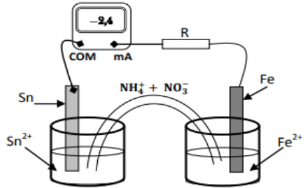
\includegraphics[width=0.3\textwidth]{./ex_00.png}
\end{center}
\end{wrapfigure}

on réalise la pile suivante avec : $S_1$ solution de sulfate d'étain(II) \\$(Sn^{2+} + SO_4^{2-})$ de concentration $C_1$=$0.5mol/L$ et $V_1=200mL$.
et  $S_2$ \\solution de sulfate de cuivre(II) $(Fe^{2+} + SO_4^{2-}$) de concentration $C_2=0.2mol/L$ \\et $V_2=200mL$. un pont salin .

on donne : $1F=96500 C/mol$ , $M(Fe)=56g/mol$

\begin{tabular}{c|l}
	0,25  & \makecell[l]{ \textbf{1. }Indiquer sur le schéma le sens du déplacement des porteurs \\de
charges.}\\
	0,25  & \makecell[l]{ \textbf{2. }Quel est le rôle du pont salin? }\\
	0,25  & \makecell[l]{ \textbf{3. }Donner le schéma conventionnel de la pile étudiée. }\\
	0,5 & \makecell[l]{ \textbf{4. }Indiquer la cathode et l’anode avec \underline{justification}}\\ 
	1 & \makecell[l]{ \textbf{5. }Ecrire les demi-équations et l’équation qui modélise le
fonctionnement de la pile}\\
	1,25	& \makecell[l]{ \textbf{6. }Calculer le temps de fonctionnement maximal de la pile pour une
intensité \\constante $I_0=0.5 A$.}\\
		2 & \makecell[l]{ \textbf{7. }On change l’intensité I et on remarque que la masse de l’électrode de fer a diminuée \\de $28mg$ pendant un
		fonctionnement de $1h15min$, \underline{calculer l’intensité I} }\\
	\end{tabular}

 \section*{Partie 2 : Evolution spontanée d'un système chimique. \dotfill(1,5pts) }

	On réalise la pile constituée des couples $(Ni^{2+}_{(aq)}/Ni_(s))$ et $(Zn^{2+}_{(aq)}/Zn_{(s)})$ en immergeant L’électrode de Nickel dans une solution de sulfate de Nickel $(Ni^{2+}_{(aq)} + SO^{2-}_{4(aq)})$ de 
	volume $V = 150 mL$ et de concentration molaire initiale $[Ni^{2+}_{(aq)}]_i=10^{-2} mol/L$.


L’électrode de Zinc dans une solution de sulfate de Zinc $(Zn^{2+}_{(aq)} +SO^{2-}_{4(aq)})$
de volume $V = 150 mL$ et de concentration molaire initiale $[Zn^{2+}_{(aq)}]_i=10^{-2} mol/L$ ,On relie les deux compartiments par un pont ionique. La constante d’équilibre associée à l’équation de la réaction suivante est $K=10^{18}$ : $$\ce{$Ni^{2+}_{(aq)}$ + $Zn_{(s)}$ <=>[1][2] $Ni_{(s)}$ + $Zn^{2+}_{(aq)}$ }$$

\begin{tabular}{c|l}
	0,5  & \makecell[l]{ \textbf{1. }Préciser, en calculant le quotient de réaction $Q_{r,i}$ à l’état initial, le sens spontané
\\d’évolution du système constituant la pile.
}\\
	0,5  & \makecell[l]{ \textbf{2. } Donner le schéma conventionnel de la pile étudiée.}\\
	0,5  & \makecell[l]{ \textbf{3. } Au cours du fonctionnement de la pile, le circuit extérieur est traversé par un
courant \\d’intensité $I = 0,1 A$. Trouver la durée maximale $\Delta{t}_{max}$ de fonctionnement de la pile en fonction\\ de : $[Zn^{2+}_{(aq)}]_i$ , V, F et I .Calculer $\Delta{t}_{max}$
 }\\
	\end{tabular}
%\hrulefill
%\Large{Physique 13pts/78min}
%\hrulefill\\
	\vspace{3cm}
\begin{center}
    %\vspace{.60cm}
\hrulefill
\Large{Physique 13pts - 78min}
\hrulefill\\
    \emph{Les  parties sont indépendantes}
\end{center}

\vspace{-1cm}
\section*{Partie 1 :  Circuit RLC série. \dotfill(7pts)}
\vspace{-0.4cm}

\begin{wrapfigure}[1]{r}{0.25\textwidth}
	\vspace{-1.2cm}
\begin{center}
  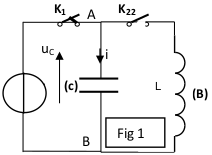
\includegraphics[width=0.25\textwidth]{./ex_011.png}
\end{center}
\end{wrapfigure}


On considère le circuit électrique schématisé dans la figure 4, comportant :

\begin{itemize}
	\item Un générateur de tension continue (G), de f.é.m $U_0$ et de résistance interne \\ négligeable, Un condensateur (c) de capacité C et d’armatures A et B ;
	\item Une bobine (B) d’inductance L et de résistance négligeable ;
	\item Deux interrupteurs $K_1$ et $K_2$.

\end{itemize}




\begin{tabular}{c|l}
	0,5& \makecell[l]{\textbf{1. }$K_2$ étant ouvert, on ferme $K_1$. Après une brève durée, le condensateur porte une charge \\maximale $Q_0$
et emmagasine une énergie électrostatique $E_0$.Donner l’expression de $Q_0$ en fonction\\ de $U_0$ et C.
et l’expression de $E_0$ en fonction de $Q_0$ et C.}\\

\end{tabular}

Le condensateur étant chargé, à t = 0 on ouvre $K_1$ et on ferme $K_2$. A t quelconque, l’armature A du
condensateur porte une charge q.

\begin{tabular}{c|l}
	0,5 & \makecell[l]{\textbf{2. }Exprimer l’énergie électromagnétique E en fonction de L, C, q et $i$.}\\

	0,5 & \makecell[l]{\textbf{3. }Montrer, sans faire aucun calcul que cette énergie se conserve et elle est égale à $\frac{Q_0^2}{2.C}$  }\\

	0,5 & \makecell[l]{\textbf{4. }Déduire l’équation différentielle des oscillations électriques.  }\\
	
	0,5 & \makecell[l]{\textbf{5. }Déterminer l’expression de la période propre $T_0$ en fonction de L et C.  }\\

	0,5 & \makecell[l]{\textbf{6. }Ecrire l’expression de la charge q en fonction du temps. }\\
	
	0,5 & \makecell[l]{\textbf{7. }Donner l’expression de l’énergie magnétique $E_L$ en fonction de L et i }\\

	1 & \makecell[l]{\textbf{8. }Montrer que l’expression de cette énergie $E_L$ en fonction du temps s’écrit :   \\\hspace{3cm}$E_L = \frac{E_0}{2}.\bigg(1+cos\big(\frac{4.\pi}{T_0}.t + \pi \big)\bigg) $ }\\
\end{tabular}

Une étude expérimentale a permis de tracer les courbes (1) et (2) (ci-dessous) traduisant
respectivement les variations de l’énergie magnétique EL en fonction de i et en fonction du temps.

\begin{center}
  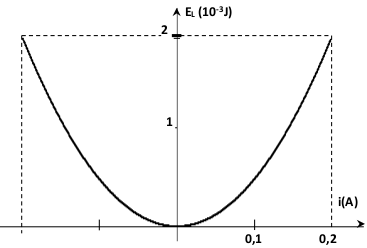
\includegraphics[width=0.43\textwidth]{./ex_01.png}
  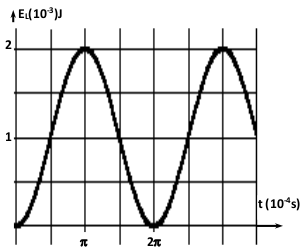
\includegraphics[width=0.33\textwidth]{./ex_02.png}
\end{center}


\begin{tabular}{c|l}
	1 & \makecell[l]{\textbf{9. }En exploitant les courbes , Déterminer la valeur de $T_0$. }\\
	1,5 & \makecell[l]{\textbf{10. }déduire la valeur de $C,Q_0$ et $U_0$ }\\


\end{tabular}



\section*{Partie 2 :  Applications: Production d'ondes électromagnétiques et
communication \dotfill(6pts)}

\begin{wrapfigure}[6]{r}{0.4\textwidth}
	\vspace{-1.2cm}
\begin{center}
  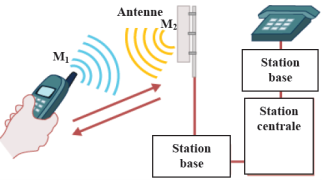
\includegraphics[width=0.4\textwidth]{./ex_031.png}
\end{center}
\vspace{-0.9cm}
\caption{}
\end{wrapfigure}



\emph{Lors d’une communication, la voix est convertie en signal électrique par un microphone, grâce à un système de
conversion numérique et d’amplification. Le signal électrique est porté par une onde porteuse qui après
amplification est émise vers l’antenne la plus proche. L’antenne transmet le signal à une station base qui
l’envoie alors à une centrale, par ligne téléphonique conventionnelle ou par les ondes électromagnétiques.}
 \\De là sont acheminées les conversations vers le
téléphone du destinataire.

\section*{1.Émission d’une onde électromagnétique par un portable}

Les ondes électromagnétiques sont utilisées par la
télévision, La radio et les radars. Si bien que la gamme de
fréquence restant pour les portables sont de plus en plus
restreints : l’une d’entre elles s’étend de 900 à 1800 MHz.

\textbf{Données : }La célérité des ondes électromagnétiques
dans le vide et dans l’air : $c = 3,00.10^8 m.s^{-1}$; $1MHz =10^6Hz$.

\begin{tabular}{c|l}
0,25 & \makecell[l]{ \textbf{1.1. }Calculer la durée que met une onde électromagnétique de fréquence $f=900MHz$ \\pour parcourir la
distance $M_1M_2=1km$ séparant le téléphone et l’antenne, figure (1). } \\

0,25& \makecell[l]{\textbf{1.2. }Que signifie l’expression \emph{l’air est un milieu dispersif pour les ondes électromagnétiques}? }\\
 0,25& \makecell[l]{ \textbf{1.3. }On peut représenter la chaine d’émission par le schéma de la figure (3).En quel point A \\ou B ou C de la figure (3) trouve-t-on L’onde porteuse ? Le signal modulant ? }\\
\end{tabular}

\begin{center}
  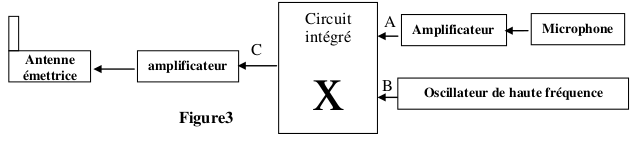
\includegraphics[width=0.8\textwidth]{./ex_032.png}
\end{center}

\section*{2.Modulation d’amplitude \dotfill }

\begin{wrapfigure}[1]{r}{0.3\textwidth}
	\vspace{-1.2cm}
\begin{center}
  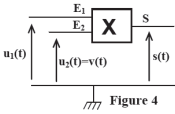
\includegraphics[width=0.3\textwidth]{./ex_033.png}
\end{center}
\end{wrapfigure}



Le circuit de modulation est constitué d’un composant nommé multiplieur
qui possède deux entrées E1 et E2 et une sortie S,

Pour simuler la modulation d’amplitude, on applique :
\begin{itemize}

	\item À l’entrée $E_1$ le signal $u_1(t)=u(t)+U_0$ dont $u(t)=U_mcos(2.\pi.f.t)$ est\\ le
signal modulant et $U_0$ tension continue de décalage .
\item À l’entrée $E_2$ le signal porteur $u_2(t)=v(t)=V_m.cos(2.\pi.F.t)$.
\item Le circuit intégré X donne une tension modulée proportionnelle
au produit des deux tensions, $s(t)$=$ k.u_1(t).u_2(t)$ où k est une
constante dépendant uniquement du circuit intégré . s(t) s’écrit
sous la forme : $s(t)$=$S_mcos(2.\pi.F.t)$.
\end{itemize}

\begin{wrapfigure}[1]{r}{0.3\textwidth}
	\vspace{-3.5cm}

\begin{center}
  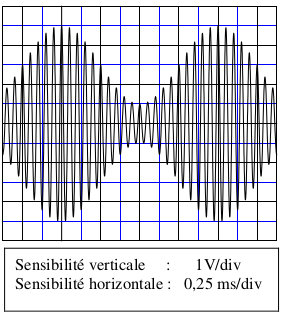
\includegraphics[width=0.3\textwidth]{./ex_034.png}
\end{center}
\end{wrapfigure}


\begin{tabular}{c|l}
	0,5 & \makecell[l]{\textbf{2.1. }Montrer que $S_m$,amplitude du signal modulé , peut se
mettre sous la forme\\ $S_m = A.\big[m.cos(2.\pi.f.t)+1\big]$ en précisant
l’expression du taux de modulation m et celle de la \\constante A . }\\
		&\makecell[l]{\textbf{2.2. }Le graphe représenté sur la figure (5) donne l’allure de la
tension modulée en fonction \\du temps. Déterminer à partir de ce
graphe : }\\
		0,25& \makecell[l]{\textbf{2.2.1. }la fréquence F de l’onde porteuse .}\\
		0,25& \makecell[l]{\textbf{2.2.2. }la fréquence $f$ de l’onde modulant .}\\
		0,25& \makecell[l]{\textbf{2.2.3. }L’amplitude minimale $S_{m(min)}$ et l’amplitude maximale \\$S_{m(max)}$ du signal modulé.}\\

		1 &\makecell[l]{\textbf{2.3. }Donner l’expression du taux de modulation en fonction \\de $S_{m(min)}$ et $S_{m(max)}$. Calculer la valeur de m . }\\

	0,5 &\makecell[l]{\textbf{2.4. }La modulation effectuée est-elle de bonne qualité ? \\Justifier. }\\

	2,5 &\makecell[l]{\textbf{2.5. }Pour une bonne réception du signal modulée, on utilise\\ un
circuit bouchon(circuit d'accord) formé d'une bobine
\\d'inductance $L_0 = 60mH$ et de résistance négligeable et
deux \\condensateurs , montés en série, de capacité $C =10\mu.F$
et $C_0$ .\\\underline{Déterminer la valeur de $C_0$?}. Tracer le disjoncteur (circuit d'accord) et \\expliquer le rôle de chaque étape ? }

\end{tabular}

\end{document}
